\documentclass[%
 reprint,
%superscriptaddress,
%groupedaddress,
%unsortedaddress,
%runinaddress,
%frontmatterverbose, 
%preprint,
%preprintnumbers,
%nofootinbib,
%nobibnotes,
%bibnotes,
 amsmath,amssymb,
 aps,
%pra,
%prb,
%rmp,
%prstab,
%prstper,
%floatfix,
]{revtex4-2}

\usepackage{graphicx}% Include figure files
\usepackage{dcolumn}% Align table columns on decimal point
\usepackage{bm}% bold math
\usepackage[breaklinks, hidelinks, colorlinks=true,linkcolor=blue,citecolor=blue]{hyperref}
%\usepackage[mathlines]{lineno}% Enable numbering of text and display math
%\linenumbers\relax % Commence numbering lines


\begin{document}



\title{Título do artigo} 

\author{Ann Author}

\author{Second Author}%
 \email{Second.Author@institution.edu}
\affiliation{%
 Authors' institution and/or address\\
 This line break forced with \textbackslash\textbackslash
}%

\author{Charlie Author}
\affiliation{
 Second institution and/or address\\
 This line break forced% with \\
}%
\affiliation{
 Third institution, the second for Charlie Author
}%

\date{\today}% It is always \today, today,
             %  but any date may be explicitly specified

\begin{abstract}
Resumo do artigo.

\end{abstract}

%\keywords{Suggested keywords}%Use showkeys class option if keyword
                              %display desired
\maketitle

%\tableofcontents

\section{Introdução}
\label{sec:level1}

Introdução do trabalho.

\subsection{Objetivos}
\label{sec:obj}

\begin{enumerate}
    \item Objetivo 1
    \item Objetivo 2...
\end{enumerate}

\section{Metodologia}
\label{sec:metodologia}

Exemplo de citação: O modelo desenvolvido por He et al. \cite{he2016deep} foi aplicado...

Exemplo de equações. 

Equação inline:

A média foi calculada como $\frac{1}{n}\sum_i x_i$. O valor foi...

Equação displayed:

A média foi calculada como

\begin{equation}
\frac{1}{n}\sum_i x_i \label{eq:media}
\end{equation}
O valor foi...

\subsection{Preparação dos dados}

Exemplo de subseção.

\section{Resultados}

Exemplo de referência cruzada: A metodologia descrita na Seção \ref{sec:metodologia} foi aplicada...

O resultado foi calculado utilizando a Equação \ref{eq:media}.

O resultado pode ser visto na Figura \ref{fig:plot}

\begin{figure}
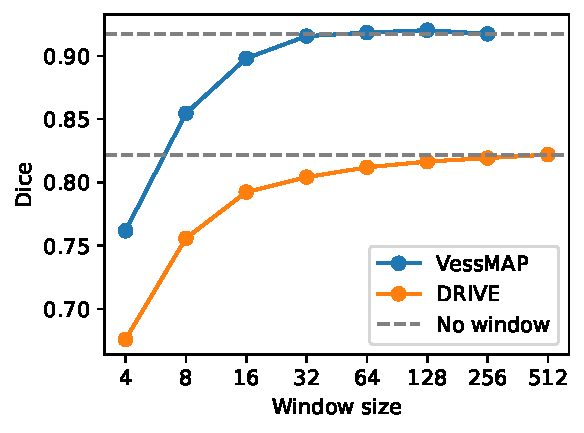
\includegraphics[width=\columnwidth]{imgs/example_plot.pdf}% Here is how to import EPS art
\caption{\label{fig:plot}Exemplo de figura de uma coluna.}
\end{figure}

\begin{figure*}
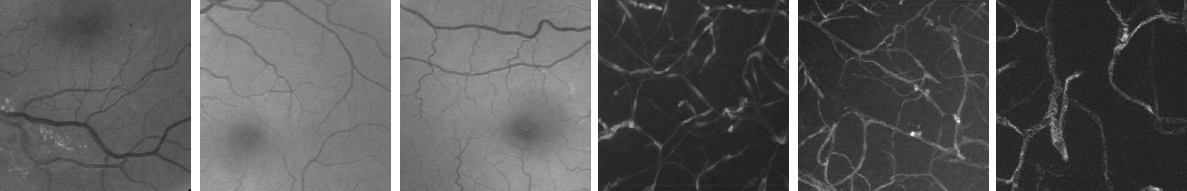
\includegraphics[width=\linewidth]{imgs/images.pdf}% Here is how to import EPS art
\caption{\label{fig:imgs} Exemplo de figura de duas colunas.}
\end{figure*}



\begin{table}[b]
\caption{\label{tab:table2}
Exemplo de tabela. Tabelas são complicadas de criar em Latex. É mais simples utilizar algum gerador online de tabelas de Latex.}
\begin{ruledtabular}
\begin{tabular}{cccccccc}
 &$r_c$ (\AA)&$r_0$ (\AA)&$\kappa r_0$&
 &$r_c$ (\AA) &$r_0$ (\AA)&$\kappa r_0$\\
\hline
Cu& 0.800 & 14.10 & 2.550 &Sn
& 0.680 & 1.870 & 3.700 \\
Ag& 0.990 & 15.90 & 2.710 &Pb
& 0.450 & 1.930 & 3.760 \\
Au& 1.150 & 15.90 & 2.710 &Ca
& 0.750 & 2.170 & 3.560 \\
Mg& 0.490 & 17.60 & 3.200 &Sr
& 0.900 & 2.370 & 3.720 \\
Zn& 0.300 & 15.20 & 2.970 &Li
& 0.380 & 1.730 & 2.830 \\
Cd& 0.530 & 17.10 & 3.160 &Na
& 0.760 & 2.110 & 3.120 \\
Hg& 0.550 & 17.80 & 3.220 &K
&  1.120 & 2.620 & 3.480 \\
Al& 0.230 & 15.80 & 3.240 &Rb
& 1.330 & 2.800 & 3.590 \\
Ga& 0.310 & 16.70 & 3.330 &Cs
& 1.420 & 3.030 & 3.740 \\
In& 0.460 & 18.40 & 3.500 &Ba
& 0.960 & 2.460 & 3.780 \\
Tl& 0.480 & 18.90 & 3.550 & & & & \\
\end{tabular}
\end{ruledtabular}
\end{table}

\section{Conclusões}

\bibliography{apssamp}% Produces the bibliography via BibTeX.

\end{document}
%
% ****** End of file apssamp.tex ******
